\documentclass[10pt,fleqn]{article} % Default font size and left-justified equations
\usepackage[%
    pdftitle={CIN : Vérification des performances cinématiques des systèmes},
    pdfauthor={Xavier Pessoles}]{hyperref}
    
\input{style/new_style}
\input{style/macros_SII}

\usepackage{multicol}
\fichetrue
%\fichefalse

\proftrue
%\proffalse

\tdtrue
%\tdfalse

\courstrue
\coursfalse

\def\discipline{Sciences \\Industrielles de \\ l'Ingénieur}
\def\xxtete{Sciences Industrielles de l'Ingénieur}

\def\classe{PTSI}
\def\xxnumpartie{Cycle 8}
\def\xxpartie{Vérification des performances cinématiques des systèmes\\
Analyser, Modéliser, Résoudre}

\def\xxnumchapitre{Chapitre 5}
\def\xxchapitre{Étude des trains épicycloïdaux}

\def\xxtitreexo{Broyeur à cisailles rotatives}
\def\xxsourceexo{\hspace{.2cm} D'après BTS CPI -- 2015.}


\def\xxposongletx{2}
\def\xxposonglettext{1.45}
\def\xxposonglety{20}
\def\xxonglet{Cycle 6 -- Ch. 5}

\def\xxactivite{Colle 1}
\def\xxauteur{\textsl{Xavier Pessoles}}

\def\xxcompetences{%
\textsl{%
\textbf{Savoirs et compétences :}\\
\noindent \textbf{Analyser :} 
\begin{itemize}[label=\ding{112},font=\color{ocre}] 
\item \textit{A3 -- C6 :} transmetteurs de puissance.
\end{itemize}
\noindent \textbf{Modéliser :} \textit{proposer un modèle de connaissance du système.}
}}

\def\xxfigures{
\includegraphics[width=.7\textwidth]{images/broyeur_01}
}%figues de la page de garde

\def\xxpied{%
Cycle 6 -- Vérification des performances cinématiques \\
Ch. 5 : Étude des trains épicycloïdaux -- \xxactivite%
}


\setcounter{secnumdepth}{5}
%---------------------------------------------------------------------------


\begin{document}
%\chapterimage{png/Fond_Cin}
\input{style/new_pagegarde}
\vspace{7cm}
\pagestyle{fancy}
\thispagestyle{plain}


\def\columnseprulecolor{\color{ocre}}
\setlength{\columnseprule}{0.4pt} 

\begin{multicols}{2}

\begin{obj}~\\
\begin{itemize}
\item Vérifier les performances d'un réducteur.
\end{itemize}
\end{obj}
ECP Group est un fabricant européen spécialisé
dans la conception et la construction de machines
permettant la réduction du volume de ces D.I.B. au
moyen de broyeurs, de compacteurs ou de presses,
en favorisant la revalorisation, le recyclage ou le réemploi
de matières.

\begin{center}
\includegraphics[width=\linewidth]{images/broyeur_04}
\end{center}

On donne un extrait du cahier des charges que doit respecter le broyeur.


\begin{center}
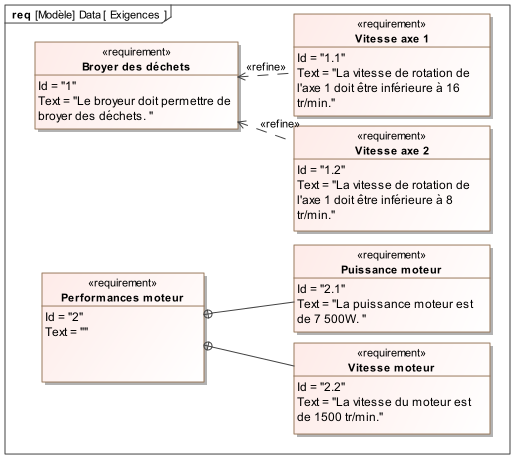
\includegraphics[width=\linewidth]{images/Exigences}
\end{center}

On donne le schéma cinématique du broyeur
\begin{center}
\includegraphics[width=\linewidth]{images/broyeur_05}
\end{center}

\subparagraph{}\textit{Donner les rapports de chacun des 4 étages de réduction.}


\subparagraph{}\textit{Vérifier que les exigences 1.1 et 1.2 sont satisfaites.}

\subparagraph{}\textit{Évaluer le couple de broyage sur chacun des axes.}



\end{multicols}

\end{document}


